\documentclass[twoside, 12pt, a4paper, openright, fleqn, cleardoublepages=empty]{scrreprt}
%%%%%%%%%%%%%%%%%%%%%%%%%%%%%%%%%%%%%%%%%%%%%%%%%%%%%%%%%%%%%%%%%%%%%%%%%%%%%%%
%%% DEFINITIONS
%%%%%%%%%%%%%%%%%%%%%%%%%%%%%%%%%%%%%%%%%%%%%%%%%%%%%%%%%%%%%%%%%%%%%%%%%%%%%%%
%Title der Arbeit
\def\myTitle{Indoor-Lokalisation}
%Vorname des Authors
\def\myAuthorFirst{Andreas}
%Nachnahme des Autors
\def\myAuthorFamily{Pfohl}
%Art der Arbeit
\def\mySeminar{Seminararbeit}
%Betreuendes Institut
\def\myInstitute{Institut f\"ur Verteilte Systeme}
%Betreuender Professor
\def\myProf{Prof. Dr. rer. nat. Kaiser}
%1. Betreuer
\def\myTutorA{Christoph Steup, Sebastian Zug}
%2. Betreuer
%\def\myTutorB{Dipl.-Inform. Betreuer2 (Affiliation)}
%Jahr der Abgabe
\def\myYear{2013}
%Sommersemester oder Wintersemester
\def\myTerm{Sommersemester}
\def\myAbstract{abstract}
% \def\myVorwort{vorwort}
% \def\myUseSourceCode{}
% \def\myAcronyms{acronyms}
\date{\today}

%Input kram, UTF-8 support, sowie deutsche Sonderzeichen
\usepackage[T1]{fontenc}
\usepackage[utf8]{inputenc}
%Deutsche Silbentrennung
\usepackage[ngerman]{babel}
%Einbinden von Grafiken
\usepackage[pdftex]{graphicx}

%PDF links
\usepackage[pdftex,plainpages=false,colorlinks,citecolor=black,linkcolor=red,urlcolor=blue,bookmarksopen]{hyperref}
%Kopf und Fußzeilen
\usepackage[automark,standardstyle,markusedcase]{scrpage2}
%Berechnungen innerhalb LATEXs
\usepackage{calc}
%Absatztrennung durch Leerzeile statt Einrückung
\usepackage{parskip}

%Deutsches Format für Referenzen
\usepackage{bibgerm}
%Support für \url, zur korrekten Darstellung von URLs
\usepackage{url}
%Erweiterte Mathesymbole
\usepackage{amssymb}
%Erweiterte Mathefunktionen
\usepackage{amsmath}
%Floating figures in figure Umgebung
\usepackage{subfig}
%Quellcode Darstellung und Formatierung
\usepackage{listings}
%Abkürzungen und Abkürzungsverzeichniss
\usepackage[printonlyused]{acronym}

\def\todoOptions{german}%, disable}

%Kommentare und Notizen während des Schreibens
\usepackage[colorinlistoftodos, \todoOptions]{todonotes}
\usepackage{color}
\usepackage{ifthen}

\newboolean{useTodos}
\setboolean{useTodos}{true}

\newcommand{\disableTodos}[0]{\setboolean{useTodos}{false}}
\newcommand{\enableTodos}[0]{\setboolean{useTodos}{true}}

\newcommand{\newRevisor}[1]{\newcounter{todoCounter-#1}\setcounter{todoCounter-#1}{1}}
\newcommand{\revisorId}[1]{#1-\arabic{todoCounter-#1}}
\newcommand{\comment}{Kommentar}
\newcommand{\error}{Fehler}
\newcommand{\rewrite}{\"Uberarbeiten}
\definecolor{bgError}{rgb}{1.0,0.5,0.5}
\definecolor{bgNote}{rgb}{0.0,1.0,0.0}
\definecolor{bgRewrite}{rgb}{1.0,1.0,0.5}

\newcommand{\thought}[1]{\ifuseTodos\todo[nolist, inline, color=green]{#1}\fi}
\newcommand{\lookup}[1]{\ifuseTodos\todo[color=yellow]{#1}\fi}
\newcommand{\doCite}[1]{\ifuseTodos\todo[color=blue!50]{#1}\fi}

\newcommand{\todoComment}[3][]{%
  \ifuseTodos%
  \todo[inline, color=green, caption={\revisorId{#2}: \comment}, #1]{\textbf{\revisorId{#2}}: #3}%
  \stepcounter{todoCounter-#2}%
  \fi%
}

\newcommand{\todoNote}[4][]{%
  \ifuseTodos%
  \todo[color=green, caption={\revisorId{#2}: \comment}, #1]{\textbf{\revisorId{#2}}: #3}%
  \stepcounter{todoCounter-#2}%
  \colorbox{bgNote}{#4}
  \else%
  #4%
  \fi%
}

\newcommand{\todoError}[4][]{%
  \ifuseTodos%
  \todo[color=red, caption={\revisorId{#2}: \error}, #1]{\textbf{\revisorId{#2}}: #3}%
  \stepcounter{todoCounter-#2}%
  \colorbox{bgError}{#4}%
  \else%
  #4%
  \fi%
}

\newcommand{\todoRewrite}[4][]{%
  \ifuseTodos%
  \todo[color=yellow, caption={\revisorId{#2}: \rewrite}, #1]{\textbf{\revisorId{#2}}: #3}%
  \stepcounter{todoCounter-#2}%
  \colorbox{bgRewrite}{#4}%
  \else%
  #4%
  \fi%
}


\newRevisor{RevisorA}
%\disableTodos

%%%%%%%%%%%%%%%%%%%%%%%%%%%%%%%%%%%%%%%%%%%%%%%%%%%%%%%%%%%%%%%%%%%%%%%%%%%%%
%%% PRIVATE PACKAGES
%%%%%%%%%%%%%%%%%%%%%%%%%%%%%%%%%%%%%%%%%%%%%%%%%%%%%%%%%%%%%%%%%%%%%%%%%%%%%
\usepackage{array,tabularx,multirow}
\usepackage{tikz}
\usetikzlibrary{calc}
\usetikzlibrary{3d}
\usetikzlibrary{positioning}
\usepackage{bytefield}
\usepackage{caption}

\hypersetup{
    pdftitle    = {\myTitle},
    pdfsubject  = {\mySeminar},
    pdfkeywords = {},
    pdfauthor   = {\textcopyright\ \myAuthorFirst\ \myAuthorFamily},
  }
\pdfcompresslevel=9

\makeatletter
\providecommand*{\toclevel@algorithm}{0}
\makeatother
\textwidth 14cm
\textheight 21cm
\headsep 3em
\headheight 1em
\evensidemargin 1cm
\oddsidemargin 1cm
\setlength{\parskip}{1.5ex plus 0.5ex minus 0.5ex}
\pagestyle{scrheadings}
\setlength{\headheight}{3\baselineskip}
\setheadsepline{.4pt}
\hyphenation{aus-zu-tauschen such-text}
\DeclareGraphicsExtensions{.jpg,.pdf,bmp,.png}


\DeclareCaptionFont{white}{\color{white}}
\DeclareCaptionFormat{listing}{\colorbox{gray}{\parbox{\textwidth}{#1#2#3}}}
\captionsetup[lstlisting]{format=listing,labelfont=white,textfont=white}

% This is 'SCHUSTER.STY' as of 25. March 1990
% Disable single lines at the start of a paragraph (Schusterjungen)
\clubpenalty = 10000
% Disable single lines at the end of a paragraph (Hurenkinder)
\widowpenalty = 10000 \displaywidowpenalty = 10000

\title{\sc \myTitle}
\author{\myAuthorFirst\ \myAuthorFamily}

%%%%%%%%%%%%%%%%%%%%%%%%%%%%%%%%%%%%%%%%%%%%%%%%%%%%%%%%%%%%%%%%%%%%%%%%%%%%%%%
%%% DOCUMENT
%%%%%%%%%%%%%%%%%%%%%%%%%%%%%%%%%%%%%%%%%%%%%%%%%%%%%%%%%%%%%%%%%%%%%%%%%%%%%%%
\begin{document}
%%%%%%%%%%%%%%%%%%%%%%%%%%%%%%%%%%%%%%%%%%%%%%%%%%%%%%%%%%%%%%%%%%%%%%%%%%%
%%% PREAMBLE
%%%%%%%%%%%%%%%%%%%%%%%%%%%%%%%%%%%%%%%%%%%%%%%%%%%%%%%%%%%%%%%%%%%%%%%%%%%
\def\HAbst{0.5cm}
\begin{titlepage}
    \begin{flushleft}
        \begin{center}
            
\includegraphics[width=14cm]{figures/signet/INF_SIGN_druck}\\[1.5cm]
            {\large \myInstitute\\}{\Large \mySeminar \\[2cm]}
            {\Large \bf \myTitle\\[0.5cm]}
            \begin{tabular}[t]{ll}
                \myTerm & \myYear\\
            \end{tabular}
        \end{center}
    \vspace*{\fill}
  \large
  \begin{tabular}[t]{ll}
    Autor:     &  \myAuthorFirst\ \myAuthorFamily  \\ & \\
    Professor:  &  \myProf    \\ & \\
    Betreuer:  &  \myTutorA  \\ & \\
    \ifdefined\myTutorB
    Betreuer:  &  \myTutorB  \\ & \\
    \fi
    \ifdefined\myTutorC
    Betreuer:  &  \myTutorC  \\ & \\
    \fi
    \ifdefined\myTutorD
    Betreuer:  &  \myTutorD  \\ & \\
    \fi
  \end{tabular}
\end{flushleft}
\newpage
\vspace*{\fill}
%    \begin{tabular}[b]{l}
%          \normalsize Universit\"at Magdeburg \\
%      \normalsize Fakult\"at f\"ur Informatik \\
%      \normalsize Postfach 4120 \\
%      \normalsize D-39016 Magdeburg \\
%      \normalsize Germany \\
%    \end{tabular}
\begin{minipage}[]{\textwidth-2cm}
  \textbf{\myAuthorFamily, \myAuthorFirst: }\emph{\myTitle}\\
  \mySeminar, Otto"=von"=Guericke"=Universit\"at\\Magdeburg, \myYear.%%TODO UNI, Institut, Addresse, Jahr
\end{minipage}
\end{titlepage}

\cleardoublepage
\sloppy
\pagenumbering{roman}

\deftripstyle{chap}[0pt][0.5pt]{}{}{}{}{\pagemark}{}
\deftripstyle{nonChap}[0pt][0.5pt]{}{}{\headmark}{}{\pagemark}{}
\renewcommand*{\chapterpagestyle}{chap}
\pagestyle{nonChap}

%%%%%%%%%%%%%%%%%%%%%%%%%%%%%%%%%%%%%%%%%%%%%%%%%%%%%%%%%%%%%%%%%%%%%%%%%%%
%%% ABSTRACT
%%%%%%%%%%%%%%%%%%%%%%%%%%%%%%%%%%%%%%%%%%%%%%%%%%%%%%%%%%%%%%%%%%%%%%%%%%%
\ifdefined\myAbstract
\chapter*{Abstrakt}
\input{\myAbstract}
\cleardoublepage
\fi

%%%%%%%%%%%%%%%%%%%%%%%%%%%%%%%%%%%%%%%%%%%%%%%%%%%%%%%%%%%%%%%%%%%%%%%%%%%
%%% PREFACE
%%%%%%%%%%%%%%%%%%%%%%%%%%%%%%%%%%%%%%%%%%%%%%%%%%%%%%%%%%%%%%%%%%%%%%%%%%%
\ifdefined\myVorwort
\chapter*{Vorwort}
\input{\myVorwort}
\cleardoublepage
\fi

%%%%%%%%%%%%%%%%%%%%%%%%%%%%%%%%%%%%%%%%%%%%%%%%%%%%%%%%%%%%%%%%%%%%%%%%%%%
%%% TABLE OF CONTENT
%%%%%%%%%%%%%%%%%%%%%%%%%%%%%%%%%%%%%%%%%%%%%%%%%%%%%%%%%%%%%%%%%%%%%%%%%%%
\renewcommand{\baselinestretch}{1.2}
\small\normalsize
\tableofcontents
\renewcommand{\baselinestretch}{1}
\small\normalsize
\cleardoublepage

%%%%%%%%%%%%%%%%%%%%%%%%%%%%%%%%%%%%%%%%%%%%%%%%%%%%%%%%%%%%%%%%%%%%%%%%%%%
%%% LIST OF FIGURES
%%%%%%%%%%%%%%%%%%%%%%%%%%%%%%%%%%%%%%%%%%%%%%%%%%%%%%%%%%%%%%%%%%%%%%%%%%%
% \renewcommand{\baselinestretch}{1.3}
% \small\normalsize
% \listoffigures
% \addcontentsline{toc}{chapter}{Abbildungsverzeichnis}
% \renewcommand{\baselinestretch}{1}
% \small\normalsize
% \cleardoublepage

%%%%%%%%%%%%%%%%%%%%%%%%%%%%%%%%%%%%%%%%%%%%%%%%%%%%%%%%%%%%%%%%%%%%%%%%%%%
%%% LIST OF TABLES
%%%%%%%%%%%%%%%%%%%%%%%%%%%%%%%%%%%%%%%%%%%%%%%%%%%%%%%%%%%%%%%%%%%%%%%%%%%
% \renewcommand{\baselinestretch}{1.3}
% \small\normalsize
% \listoftables
% \addcontentsline{toc}{chapter}{Tabellenverzeichnis}
% \renewcommand{\baselinestretch}{1}
% \small\normalsize
% \cleardoublepage

%%%%%%%%%%%%%%%%%%%%%%%%%%%%%%%%%%%%%%%%%%%%%%%%%%%%%%%%%%%%%%%%%%%%%%%%%%%
%%% LIST OF LISTINGS
%%%%%%%%%%%%%%%%%%%%%%%%%%%%%%%%%%%%%%%%%%%%%%%%%%%%%%%%%%%%%%%%%%%%%%%%%%%
\ifdefined\myUseSourceCode
\renewcommand{\baselinestretch}{1.3}
\small\normalsize
\renewcommand\lstlistlistingname{Quellcodeverzeichnis}
\lstlistoflistings
\addcontentsline{toc}{chapter}{Quellcodeverzeichnis}
\renewcommand{\baselinestretch}{1}
\small\normalsize
\cleardoublepage
\fi

%%%%%%%%%%%%%%%%%%%%%%%%%%%%%%%%%%%%%%%%%%%%%%%%%%%%%%%%%%%%%%%%%%%%%%%%%%%
%%% LIST OF ACRONYMS
%%%%%%%%%%%%%%%%%%%%%%%%%%%%%%%%%%%%%%%%%%%%%%%%%%%%%%%%%%%%%%%%%%%%%%%%%%%
\ifdefined\myAcronyms
\renewcommand{\baselinestretch}{1.3}
\small\normalsize
\chapter*{Abkürzungsverzeichnis}
\input{\myAcronyms}
%\lstlistoflistings
\addcontentsline{toc}{chapter}{Abkürzungsverzeichnis}
\renewcommand{\baselinestretch}{1}
\small\normalsize
\cleardoublepage
\fi

%%%%%%%%%%%%%%%%%%%%%%%%%%%%%%%%%%%%%%%%%%%%%%%%%%%%%%%%%%%%%%%%%%%%%%%%%%%
%%% OPEN TODOS
%%%%%%%%%%%%%%%%%%%%%%%%%%%%%%%%%%%%%%%%%%%%%%%%%%%%%%%%%%%%%%%%%%%%%%%%%%%
% \renewcommand{\baselinestretch}{1.3}
% \small\normalsize
% \listoftodos
% \addcontentsline{toc}{chapter}{Todo-Verzeichnis}
% \renewcommand{\baselinestretch}{1}
% \small\normalsize
% \cleardoublepage

%%%%%%%%%%%%%%%%%%%%%%%%%%%%%%%%%%%%%%%%%%%%%%%%%%%%%%%%%%%%%%%%%%%%%%%%%%%
%%% CONTENT
%%%%%%%%%%%%%%%%%%%%%%%%%%%%%%%%%%%%%%%%%%%%%%%%%%%%%%%%%%%%%%%%%%%%%%%%%%%
\pagenumbering{arabic}
\setcounter{page}{1}
\pagestyle{scrheadings}

%% vim:tw=78:ai:bg=light:set spell:spelllang=de:set nu
%%%%%%%%%%%%%%%%%%%%%%%%%%%%%%%%%%%%%%%%%%%%%%%%%%%%%%%%%%%%%%%%%%%%%%%%%%%%
%%% Einleitung
%%%%%%%%%%%%%%%%%%%%%%%%%%%%%%%%%%%%%%%%%%%%%%%%%%%%%%%%%%%%%%%%%%%%%%%%%%%%
\chapter{Einleitung}
Positionsbestimmung in geschlossenen Räumen gewinnt immer mehr an Bedeutung.
Gerade auch in Bezug auf die Heimautomatisierung oder den Betrieb von
selbsständig arbeitenden Lagersystemen. Dabei gibt es viele Aspekte zu
beachten. Darunter fällen die Kosten, die Genauigkeit und Anwendbarkeit.
Dazu sollten verschiedene Systeme betrachtet werden um abschätzen zu können
welches System das jeweils passendste ist.

%%%%%%%%%%%%%%%%%%%%%%%%%%%%%%%%%%%%%%%%%%%%%%%%%%%%%%%%%%%%%%%%%%%%%%%%%%%%
\cleardoublepage

% vim:tw=78:ai:bg=light:set spell:spelllang=de:set nu
%%%%%%%%%%%%%%%%%%%%%%%%%%%%%%%%%%%%%%%%%%%%%%%%%%%%%%%%%%%%%%%%%%%%%%%%%%%%
%%% Lokalisierungsmethoden
%%%%%%%%%%%%%%%%%%%%%%%%%%%%%%%%%%%%%%%%%%%%%%%%%%%%%%%%%%%%%%%%%%%%%%%%%%%%
\chapter{Lokalisierungsmethoden}

\section{Globales Navigationssatellitensystem}
Das wohl bekannteste Verfahren eine Position zu ermitteln ist derzeit das
\dq Global Navigation Satellite System\dq. Der Kern dieses Systems sind Satelliten im Erdorbit, die
kontinuierlich Funksignale zur Erde senden. Diese werden dort von einem
entsprechenden Empfänger aufgenommen und mit Hilfe von mathematischen
Berechnungen zu einer globalen Position vereinigt.

Soll dieses Verfahren jedoch verwendet werden um eine Indoor-Lokalisierung
zu realisieren, steht man vor mehreren Problemen. Die
Funksignale der Satelliten sind durch Hindernisse nur noch recht schlecht
empfangbar, da deren Intensität je nach Material abnimmt. Um die Signale
einigermaßen gut empfangen zu können, werden spezielle Sensoren benötigt, was
auch einen höheren Geldaufwand bedeutet.

Ein weiteres Problem ist die große Ungenauigkeit von GNSS in Räumen. Auf Grund
von Reflexionen entstehen Fehler, die zu einer Ungenauigkeit in der
Lokalisierung führen. Die Anforderung von Lokalisierung in Räumen verlangt
eine recht hohe Auflösung, da im Verhältnis zu Draußen oft nur wenig Zeit
zum Reagieren bleibt und die Abmaße der Gebiete viel kleiner sind. Da ist
eine Abweichung von mehreren Metern nicht hinnehmbar. GNSS würde sich also
nur anbieten, wenn es darum geht, zu bestimmen in welchem Raum man sich
befindet. Um dabei eine schnelle Positionierung zu erreichen, wird das
\dq Assisted Global Positioning System\dq{} verwendet. Dabei verfügt der Empfänger über eine Datenverbindung
zu einer Informationsquelle in der Informationen darüber zufinden sind,
wo sich zum aktuellen Zeitpunkt welche Satelliten befinden. Er bekommt somit
eine hilfreiche Information, die er sonst über die Signale der Satelliten
selbst berechnen müsste. Um in Räumen eine Aussage darüber treffen zu können,
ob ein empfangenes Signal gültig ist, wird über mehrere Intervalle integriert.

\section{Vorgetäuschtes GNSS}
Bei vorgetäuschtem GNSS werden spezielle Transceiver aufgestellt, die
GNSS-ähnliche Signale aussenden. Die Transceiver sind dabei
zeitsynchronisiert. Dieses System kann sowohl indoor als auch outdoor
verwendet werden. Es erreicht dabei eine eine maximale Abweichung von
$\pm$20 mm. In Gebäuden eignet sich dieses System sehr gut für eine
Lokalisierung, da die Signale eine ausreichende Intensität haben um Wände
zu durchdringen. Indoor wird dabei jedoch nur eine Genauigkeit im
Dezimeterbereich erzielt.

\section{Laserverfolgung}
Bei diesem Verfahren werden die Objekte, von denen die Positionen
bestimmt werden sollen, mit Reflektoren ausgestattet und dann von einem
Laserinterferometer verfolgt. Aus den gesammelten Daten kann dann eine
Position bestimmt werden. Das Prinzip ist ähnlich dem der Landvermessung.
Die Reichweite kann bei der Laserverfolgung bis zu 70m betragen. Zusätzlich
besteht die Möglichkeit bewegte Objekte dauerhaft zu verfolgen, um eine
kontinuierliche Positionsbestimmung zu gewährleisten. Die Genauigkeit liegt
bei 0,001 Zoll.

\section{Funksignale}
Um Funksignale für die Lokalisierung zu verwenden, gibt es mehrere Ansätze.
Alle haben gemeinsam, dass Sender und Empfängerknoten verwendet werden. Dies
ist in zwei Richtungen möglich. Bei der ersten werden Sender im Raum verteilt
und der Empfänger bewegt sich. Die zweite Methode ist genau umgekehrt, hier
bewegt sich der Sender und wird von verteilten Empfängern wahrgenommen.

Die erste Methode ist die Laufzeitmessung der Signale. Da man die
Geschwindigkeit der Signale kennt, ist es möglich daraus die Distanz zwischen
Sender und Empfänger zu berechnen. Mit diesen Daten ist eine Triangulation
möglich.

Die zweite Methode ist die, die Ankunftsrichtung der Signale zu messen. Dazu werden
Empfänger benötigt, die eine Information darüber geben können aus welcher
Richtung Signale auftreffen.

Die beiden eben genannten Verfahren haben jedoch die Nachteile, das entweder
eine aufwendige Sensorhardware benötigt wird oder eine besondere Synchronisation
zwischen Sender und Empfänger voraus gesetzt werden muss. Um diesen Problemen
aus dem Weg zu gehen, haben Forscher der Princton University ein Verfahren
betrachtet, dass auf Basis der Signalstärke arbeitet. Bei diesem Versuch
wurden WLAN-Access-Points als Sender und Empfänger verwendet. Dabei wurden
die Entfernungen und ihre entsprechenden Signalstärken einmal empirisch
bestimmt und dann durch mathematische Methoden berechnet. Der Vorteil ist,
dass außer aufwendiger Berechnungen keine teure Hardware benötigt wurde.

%%%%%%%%%%%%%%%%%%%%%%%%%%%%%%%%%%%%%%%%%%%%%%%%%%%%%%%%%%%%%%%%%%%%%%%%%%%%
\cleardoublepage

% vim:tw=78:ai:bg=light:set spell:spelllang=de:set nu
%%%%%%%%%%%%%%%%%%%%%%%%%%%%%%%%%%%%%%%%%%%%%%%%%%%%%%%%%%%%%%%%%%%%%%%%%%%%
%%% Ultraschall
%%%%%%%%%%%%%%%%%%%%%%%%%%%%%%%%%%%%%%%%%%%%%%%%%%%%%%%%%%%%%%%%%%%%%%%%%%%%
\chapter{Ultraschall}
Die Ultraschalllokalisation benutzt die Laufzeit von Schallsignalen um
Entfernungen zu bestimmen. Um aus Entfernungen Rückschlüsse auf eine
Position ziehen zu können, werden mehrere verschiedene Strecken und Längen
benötigt. Aus diesen kann mit Hilfe der Triangulation ein Objekt lokalisiert
werden. Dabei gibt es im wesentlichen zwei Ansätze. Zum einen gibt es den
Ansatz, der \dq Sprechenden Infrastruktur\dq, bei dem das zu lokalisierende Objekt
einen Empfänger darstellt, der Signale von Beacons aufnimmt. Der andere
Ansatz ist genau umgekehrt, man spricht von \dq Sprechenden Knoten\dq.

\section{Sprechende Infrastruktur}
Wie der Name schon andeutet, wird bei diesem Verfahren ein System verwendet,
welches von vielen Stellen Ultraschallimpulse in der Raum sendet. Zusätzlich
wird ein RF-Signal von jedem Beacon ausgesandt, das den Zeitpunkt des
Absendens eines Ultraschallimpulses und das Muster des Impulses beinhaltet.
Da RF-Signale signifikant schneller sind als Ultraschallimpulse, weiß das
Objekt über den eintreffenden Ultraschallimpuls schon bescheid, bevor dieser
eintrifft. Auf Grund der Kenntnis des Absendezeitpunktes des
Ultraschallimpulses kann somit die Entfernung des Objekts zum Beacon
berechnet werden.

Um eine ausreichend genaue Lokalisation zu erzielen, müssen viele dieser
Beacons installiert werden. Durch Trilateration kann aus den bekannten
Koordinaten der Beacons und der gemessenen Entfernungen die Position
bestimmt werden.

Ein sehr bekanntes System nennt sich Cricket, welches am Massachusetts
Institute of Technology entwickelt
wurde. Cricket erreicht eine Genauigkeit von 1-2 cm auf 10 m Entfernung.
Die Cricket-Einheit kann sowohl als Beacon, als auch als Empfänger
konfiguriert werden und arbeitet mit einer Updaterate von einem Hz.

\section{Sprechender Knoten}
Das System des \dq sprechenden Knotens\dq{} arbeitet im Gegensatz zu dem der
\dq Sprechenden Infrastruktur\dq{} nach dem umgekehrten Prinzip. Die
Hauptrolle spielt hierbei ein bewegter Beacon der kontinuierlich
Ultraschallimpulse erzeugt. Das Gegenstück ist ein Netzwerk von sehr präzise
positionierten Empfängern, die das Signal des Beacons auffangen. Die
Berechnung der Position wird hier im Grunde genauso bestimmt wie bei der
\dq Sprechenden Infrastruktur\dq{}, es wird die Zeit gemessen, die der
Ultraschallimpuls vom Beacon zum Empfänger braucht. Durch die vielen
Empfänger lässt sich sehr gut eine 3D-Position bestimmen.

Ein Vorreiter auf diesem Gebiet ist das \dq Active Bat\dq -System. Seine
Genauigkeit bei der Lokalisierung liegt bei 2 cm und im 3D-Bereich bei 5 cm.

\section{Unterschied}
Der Unterschied der beiden Methoden ist, wo die Berechnung der Lokalisation
statt findet. Die Methode \dq Sprechende Infrastruktur\dq{} eignet sich dabei
sehr gut, um einen bewegten Empfänger die Möglichkeit zugeben sich selbst in
einer entsprechenden Umgebung zu Lokalisieren. Bei der Methode
\dq Sprechender Knoten\dq{} wird die Berechnung jedoch außerhalb des bewegten
Objektes vorgenommen. Damit kann ein sendendes Objekt in einem dafür
ausgestattetem Raum lokalisiert werden.

\section{Triangulation}
Da die Schallgeschwindigkeit bekannt ist, kann über die Laufzeit des
Ultraschallimpulses die Entfernung zwischen dem Beacon $O$ und den
Empfängern $S_1$ und $S_2$ berechnet werden. Wenn wir von 20 $^\circ$C warmer
Luft ausgehen, beträgt die Schallgeschwindigkeit somit 343 m/s. Die Entfernung
kann mit Hilfe des Gesetzes für die gleichförmige Bewegung berechnet werden.

\begin{equation}
  d = v\cdot t
\end{equation}

Dabei ist $d$ die Entfernung zwischen dem Beacon $O$ und dem Empfänger,
$v$ die Schallgeschwindigkeit und $t$ die Impulslaufzeit.

Allerdings kann mit einer gemessenen Entfernung, nicht die genaue Position des
Beacons bestimmt werden. Mit einer zweiten Entfernung
kann jedoch die Position über eine Dreiecksbildung bestimmt werden.
Dieses Problem wird in Abbildung 2.1 dargestellt.

\begin{figure}[htbp]
  \centering
  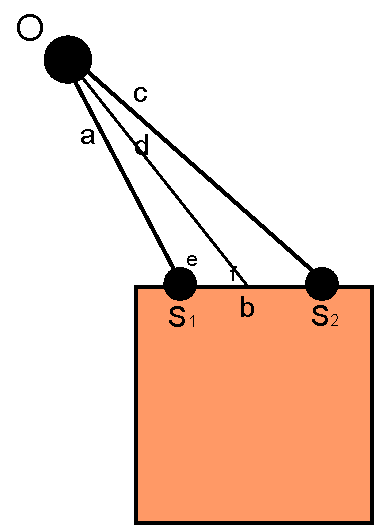
\includegraphics{figures/triangulation.pdf}
  \caption{Triangulation}
\end{figure}

Die beiden Empfänger $S_1$ und $S_2$ mit dem Abstand $b$, nehmen jeweils eine
Entfernung zum Beacon $O$ wahr. Je nachdem, welche der beiden
Entfernungen $a$ oder $c$ größer ist, kann entschieden werden, ob
sich der Beacon links oder rechts der Hauptachse der Empfänger
befindet. Um nun die tatsächliche Entfernung $d$ von der Mitte der
Sensoren und den genauen Winkel $f$ zum Beacon zu berechnen, kann der
Kosinussatz verwendet werden.

\begin{equation}
  c^2 = a^2 + b^2 - 2ab\cdot cos(\gamma)
\end{equation}

Zunächst wird der Winkel $e$ berechnet.

\begin{equation}
  e = acos\left(\frac{c^2 - a^2 - b^2}{-2ab}\right)
\end{equation}

Mit dem Winkel $e$ kann nun die exakte Entfernung $d$ von den Empfängern
zum Beacon berechnet werden.

\begin{equation}
  d = \sqrt{a^2 + \left(\frac{b}{2}\right)^2 - 2ab\cdot cos(e)}
\end{equation}

$f$ ist der Peilungswinkel von der Empfängerhauptachse zum Beacon. Der
Peilungswinkel gibt an, um wie viel Grad sich die Position des Beacons ändern müsste,
um genau Senkrecht zu den Empfängern zu stehen. Er lässt sich ebenfalls durch
den Kosinussatz berechnen.

\begin{equation}
  f = acos\left( \frac{a^2 - \left(\frac{b}{2}\right)^2 - d^2}{-bd} \right)
\end{equation}

Mit diesen beiden Werten $f$ und $d$ ist es jetzt möglich, die genaue
Position des Beacons zu bestimmen.

Diese Rechnung ist nur ein Beispiel dafür, wie Triangulation funktioniert.
Zwei Entfernungen reichen natürlich nicht aus, um eine ausreichende
Lokalisierung zu erhalten.

\section{Probleme}
Die Ultraschalltechnologie hat jedoch ein paar starke Nachteile. Die
Schallgeschwindigkeit ist abhängig von der Lufttemperatur. Bei der
Laufzeitmessung der Signale muss das berücksichtigt werden, indem eine
zusätzliche Information über die Temperatur mitgesendet werden muss. Das
wiederum macht den Aufbau des Senders oder Empfängers aufwendiger, da diese
mit einem Temperatursender ausgestattet werden müssen. Eine weitere
Möglichkeit wäre die Temperaturen separat zu messen und über ein Datennetz
zu verteilen.

Ein weiteres Problem sind Reflexionen der Ultraschallimpulse an glatten
Wänden. Es entstehen \dq Multipfadsignale\dq{} die den Empfänger verwirren
können. Es muss sichergestellt werden, dass die Signale zugeordnet werden
können. Zum Beispiel mit einem mitgesendeten RF-Signal.

Des Weiteren besteht die Möglichkeit, dass Ultraschallimpule verdeckt werden.
Wenn sich ein Beacon in meinem Raum mit vielen Störquellen befindet, z.B.
Menschen oder großen Geräten, kann es passieren, dass Impulse verloren gehen,
weil sie vorher von einem anderen Objekt absorbiert wurden. Um dem zu
begegnen, wäre es denkbar, den Bewegungspfad zu Interpolieren und durch
Messungen zu korrigieren. So fällt ein Ausfall nicht groß ins Gewicht.

\section{Vorteile}
Ein großer Vorteil in der Nutzung von Ultraschall ist die bereits sehr gute
Erforschung. Es gibt sehr viele Untersuchungen zu den verschiedensten
Aspekten. Ultraschallsender und Empfänger sind darüberhinaus auch nicht so
Kostenintensiv wie z.B. Laser oder besonders hochwertige GPS-Empfänger für
Indoor-Applikationen. Der Aufwand, um aus den Laufzeitdaten eine Position zu
berechnen ist zu dem viel geringer als z.B. die der Lokalisation durch
Funksignalstärke.

%%%%%%%%%%%%%%%%%%%%%%%%%%%%%%%%%%%%%%%%%%%%%%%%%%%%%%%%%%%%%%%%%%%%%%%%%%%%
\cleardoublepage

% vim:tw=78:ai:bg=light:set spell:spelllang=de:set nu
%%%%%%%%%%%%%%%%%%%%%%%%%%%%%%%%%%%%%%%%%%%%%%%%%%%%%%%%%%%%%%%%%%%%%%%%%%%%
%%% Fazit
%%%%%%%%%%%%%%%%%%%%%%%%%%%%%%%%%%%%%%%%%%%%%%%%%%%%%%%%%%%%%%%%%%%%%%%%%%%%
\chapter{Fazit}
Es gibt viele Möglichkeiten eine Indoor-Lokalisation auf die Beine zu
stellen. Je nach benötigter Präzision kann ein entsprechendes System
ausgewählt werden. Bei sehr geringer Präzision kann man sogar noch mit AGPS
arbeiten, wenn es nur darum geht einen Raum zu lokalisieren. Bei hoher
benötigter Präzision, wie beispielsweise beim Indoorflug, kann man auf
lasergestützes Tracking zurückgreifen.

Einen guten Mittelweg nimmt jedoch die ultraschallbasierte Lokalisation.
Sie ist genügend genau für die meisten Indoor-Anwendungen und bietet zu dem
noch zwei verschiedene Einsatzmöglichkeiten.
\dq Sprechende Infrastruktur\dq{} und \dq Sprechender Knoten\dq{} lassen
sich durchaus mit der selben Hardware realisieren.

%%%%%%%%%%%%%%%%%%%%%%%%%%%%%%%%%%%%%%%%%%%%%%%%%%%%%%%%%%%%%%%%%%%%%%%%%%%%
\cleardoublepage


%%%%%%%%%%%%%%%%%%%%%%%%%%%%%%%%%%%%%%%%%%%%%%%%%%%%%%%%%%%%%%%%%%%%%%%%%%%
%%% APPENDIX
%%%%%%%%%%%%%%%%%%%%%%%%%%%%%%%%%%%%%%%%%%%%%%%%%%%%%%%%%%%%%%%%%%%%%%%%%%%
%\begin{appendix}
%  \input{chapter/apendix_A}
%  \input{chapter/apendix_B}
%\end{appendix}

%%%%%%%%%%%%%%%%%%%%%%%%%%%%%%%%%%%%%%%%%%%%%%%%%%%%%%%%%%%%%%%%%%%%%%%%%%%
%%% BIBLIOGRAPY
%%%%%%%%%%%%%%%%%%%%%%%%%%%%%%%%%%%%%%%%%%%%%%%%%%%%%%%%%%%%%%%%%%%%%%%%%%%
\cleardoublepage
\nocite*
\bibliography{bib/references}
\bibliographystyle{geralpha}
\addcontentsline{toc}{chapter}{Literaturverzeichnis}
\cleardoublepage

% %%%%%%%%%%%%%%%%%%%%%%%%%%%%%%%%%%%%%%%%%%%%%%%%%%%%%%%%%%%%%%%%%%%%%%%%%%%%%
% %%% Selbständigkeitserklärung
% %%%%%%%%%%%%%%%%%%%%%%%%%%%%%%%%%%%%%%%%%%%%%%%%%%%%%%%%%%%%%%%%%%%%%%%%%%%%%
% \pagestyle{empty}
% \chapter*{Selbstst\"andigkeitserkl\"arung}
%
% Ich erkl\"are hiermit an Eides Statt, dass ich die vorliegende Arbeit
% selbst\"andig und ohne Benutzung anderer als der angegebenen Hilfsmittel
% angefertigt habe. Die aus fremden Quellen direkt oder indirekt \"ubernommenen
% Gedanken sind als solche kenntlich gemacht.
%
% Diese Arbeit wurde bisher weder in gleicher noch in \"ahnlicher Form einer
% anderen Pr\"ufungsbeh\"orde vorgelegt und auch noch nicht ver\"offentlicht.
%
% \vspace*{1.5cm}Magdeburg, den \today
% \hspace*{\fill}\myAuthorFirst\ \myAuthorFamily

%%%%%%%%%%%%%%%%%%%%%%%%%%%%%%%%%%%%%%%%%%%%%%%%%%%%%%%%%%%%%%%%%%%%%%%%%%%%%
%%% Ende
%%%%%%%%%%%%%%%%%%%%%%%%%%%%%%%%%%%%%%%%%%%%%%%%%%%%%%%%%%%%%%%%%%%%%%%%%%%%%
\end{document}
